\documentclass[12pt,fleqn]{article}\usepackage{../common}
\begin{document}
Dunya Kupasi 2014 Tahminleri

Projede kullanilan 4 Python dosyasi var: 

\verb!match_stats!: Mac istatistiklerini yukleyen kodlar.

\verb!features!: Ham istatistik verileri ozelliklere (features) donduruyor,
ki bu ozellikler yapay ogrenim modeline girilebilsin. Bu ozellikler onceki
K macin verilerini ozetleme amacli yaratildilar, ki bu ozelliklere
dayanarak bir sonraki maci tahmnin edebilelim.

\verb!world_cup!: Veriyi temizlemek ve modeli kurmak icin kullanilan
yardimci kodlar.

\verb!power!: Birbiriyle belli sayida mac yapmis takimlarin bir ``guc
siralamasini'' hesaplamak. 

Ozellik insasi

Sonraki mac tahmini icin onceki K macin ozet istatistiklerine bakiyoruz, K'nin
ne oldugu \verb!history_size! ile tanimli.

\begin{minted}[fontsize=\footnotesize]{python}
import world_cup
import features
import match_stats
import pandas as pd

history_size = 3

game_summaries = features.get_game_summaries()
data = features.get_features(history_size)
\end{minted}

Bu ozellikler, dedigimiz gibi, onceki K macin ozeti. Bu ozetlerin cogu bir
ortalamadir, ayrica bu ortalamalarin cogu dakika bazli cunku mac zamanini
asan maclari da hesaba katmak icin.. Eger mac basina yapilan pas degeri
alinsaydi, o zaman vakti asan bir macta o deger normalden cok daha fazla
olacakti, bu modeli bozardi.

Modelde kullanilacak ozellikler:

\verb!is_home!: Takim evinde mi, deplasmanda mi oynuyor. Futbolda bu
degiskeninin cok onemli oldugunu anladik.

\verb!avg_points!: Onceki K macta kazanilan ortalama puan (galibiyet icin
3, esitlik icin 1, kayip icin 0). 

\verb!avg_goals!: Onceki K macta atilan averaj gol.

\verb!op_average_goals!: Rakip tarafindan son K macta atilan averaj gol.

\verb!pass_70/80!: Hucum sahasinin 30\%-20\%'sinde dakika basina verilen
basarili pas.

\verb!op_pass70/80!: Hucum sahasinin 30\%-20\%'sinde rakip tarafindan
verilmis dakika bazinda basarili paslar.

\verb!expected_goals!: Son K mactaki gol beklentisi, ki bu beklenti atilan
sut ve ve sutun kaleden uzakligi baz alinarak hesaplanan bir sayi.

\verb!passes!: Dakika basina atilan paslar.

\verb!bad_passes!: Dakika bazinda verilen ama basarili olmayan paslar.

\verb!pass_ratio!: Basarili paslarin orani.

\verb!corners!: Dakika bazinda atilan kornerler.

\verb!fouls!: Yapilan faul sayisi (dk bazli)

\verb!cards!: Kirmizi ya da sari alinan kart ceza sayisi (mac basina).

\verb!shots!: Dakika bazinda atilan sut.

\verb!op_*!: Rakipler hakkindaki bazi tarihi istatistikler. Dikkat, bu
``rakip'' \verb!op_team_name!'de gosterilen rakip degil, genel olarak bu
takimin rakiplerinin ona karsi nasil oynadigini gostermeye calisan bir
istatistik. Mesela \verb!op_corners! bu takimin rakiplerinin dakika basina
kac korner kazandigini gosteriyor.

\verb!*_op_ratio!: Takimin istatistiklerinin rakiplerine olan orani [?]

Ozellik olmayan kolonlar

\verb!matchid!: Macin id'si

\verb!teamid!: Takimin id'si

\verb!op_teamid!: Rakip takimin tekil id'si

\verb!team_name!: Takimin ismi

\verb!op_team_name!: Rakip takimin ismi

\verb!timestamp!: Mac ne zaman oynandi

\verb!competitionid!: Genel musabakayi gosteren kod (dunya kupasi, vs).

Hedef kolonlar:

Alttaki kolonlar tahmin edilmeye ugrasilabilecek olan kolonlar. Eger
bilinen veri uzerinde tahmin yapmak istiyorsak, bu kolonlari tahmin oncesi
disari atmaliyiz, bunu unutmayalim. Birkac hedef kolon var ama, biz
sadece kazanilan puani tahmin etmeye ugrasacagiz, belki diger modeller
diger kolonlari tahmin etmeye ugrasirlar, mesela atilan gol sayisi gibi.

\verb!points!: Macin puan sonucu.

\verb!goals!: \verb!teamid!'deki takimin attigi gol sayisi.

\verb!op_goals!: \verb!op_teamid! ile gosterilen takimin attigi gol sayisi.

\begin{minted}[fontsize=\footnotesize]{python}
club_data = data[data['competitionid'] <> 4]
# Show the features latest game in competition id 4, which is the world cup.
print data[data['competitionid'] == 4].iloc[0]
\end{minted}

\begin{verbatim}
matchid                                  731828
teamid                                      366
op_teamid                                   632
competitionid                                 4
seasonid                                   2013
is_home                                       0
team_name                           Netherlands
op_team_name                          Argentina
timestamp            2014-07-09 21:00:00.000000
goals                                         0
op_goals                                      0
points                                        1
avg_points                             2.333333
avg_goals                              1.333333
op_avg_goals                          0.3333333
pass_70                               0.4720355
pass_80                               0.1506976
op_pass_70                            0.2647796
op_pass_80                           0.07850102
expected_goals                         1.444374
op_expected_goals                     0.4114247
passes                                 3.834864
bad_passes                             1.013622
pass_ratio                            0.7655947
corners                              0.07099121
fouls                                 0.1262374
cards                                         1
shots                                 0.1552259
op_passes                               3.38986
op_bad_passes                          1.024551
op_corners                           0.03467955
op_fouls                              0.1570661
op_cards                               2.666667
op_shots                             0.09249659
goals_op_ratio                         1.333333
shots_op_ratio                         1.702273
pass_op_ratio                          1.025426
Name: 0, dtype: object
\end{verbatim}

Mac bazinda atilan goller ve macin sonucunu eksenlere alarak bir tablo
yaratalim (crosstab).

\begin{minted}[fontsize=\footnotesize]{python}
import pandas as pd
print pd.crosstab(
    club_data['goals'], 
    club_data.replace(
        {'points': {
            0: 'lose', 1: 'tie', 3: 'win'}})['points'])
\end{minted}

\begin{verbatim}
points  lose  tie  win
goals                 
0        768  279    0
1        508  416  334
2        134  218  531
3         23   42  325
4          2    6  158
5          0    2   67
6          0    0   13
7          0    0    6
8          0    0    1
\end{verbatim}

5'den fazla gol atmak tabii ki kazanmayi garantiliyor, hic atmamak 75\%
ihtimalle kaybedilecek demektir (bazen de beraberlik olur tabii!). Not:
Fakat tabloda 4 gol sonrasi kazanimlar direk artmiyor, niye? Cunku bu
maclar uzatma sonrasi atilan penaltilardan geliyor, her iki takimda bu
sirada cok gol atiyor, ve biri mutlaka kaybediyor [1].

Modeli egitmek

Veri tabanimizdaki klup verisini kullanarak (yani hic dunya kupasi verisi
kullanmadan) egitecegiz. Bu kod  \verb!world_cup.py! icinde. Sonuc bir
lojistik regresyon modeli olacak, ve sonra test verisi uzerinde tahmin
yapacagiz. Regresyonun Rsquared degerini gosterecegiz, ki bu egitim
verisi uzerinden gosterilebilir. Rsquared modelin veriye ne kadar uydugunu
gosteren bir rakamdir, ne kadar yuksekse o kadar iyidir.

\begin{minted}[fontsize=\footnotesize]{python}
import world_cup
reload(world_cup)
import match_stats
pd.set_option('display.width', 80)

# Don't train on games that ended in a draw, since they have less signal.
train = club_data.loc[club_data['points'] <> 1] 
# train = club_data

(model, test) = world_cup.train_model(
     train, match_stats.get_non_feature_columns())
print "Rsquared: %0.03g" % model.prsquared
\end{minted}

\begin{verbatim}
Rsquared: 0.149
\end{verbatim}

Onemli ozellikleri secmek

Lojistik regresyon modelimiz regularizasyon kullaniyor; bu demektir ki daha
cetrefil modeller cezalandiriliyor. Bu cezalandirmanin yan etkisi olarak
biz hangi ozelliklerin daha onemli oldugunu gorebiliyoruz, cunku daha
onemsiz olan ozellikler modelden atiliyorlar (katsayilari sifira iniyor). 

Bu baglamda ozellikleri uce ayirabiliriz:

Pozitif ozellikler: Bu ozellikler mevcut ise takimin kazanma sansi yukseliyor.

Negative ozellikler: Tam tersi

Atilan degerler: Onemli olmayan ozellikler, ki bu ozellikler modele dahil
edilirse asiri uygunluk (overfitting) durumu ortaya cikar. 

\begin{minted}[fontsize=\footnotesize]{python}
def print_params(model, limit=None):    
    params = model.params.copy()
    params.sort(ascending=False)
    del params['intercept']
    
    if not limit:
        limit = len(params)

    print("Pozitif ozellikler")
    params.sort(ascending=False)
    print np.exp(params[[param > 0.001 for param in params]]).sub(1)[:limit]

    print("\nAtilan ozellikler")
    print params[[param  == 0.0 for param in params]][:limit]

    print("\nNegatif ozellikler")
    params.sort(ascending=True)
    print np.exp(params[[param < -0.001 for param in params]]).sub(1)[:limit]

print_params(model, 10)
\end{minted}

\begin{verbatim}
Pozitif ozellikler
is_home           0.848337
pass_70           0.254729
expected_goals    0.169235
opp_op_corners    0.159163
op_passes         0.120319
opp_op_pass_80    0.095970
avg_goals         0.092000
opp_bad_passes    0.075657
opp_cards         0.068903
fouls             0.062809
dtype: float64

Atilan ozellikler
op_pass_70            0
opp_op_cards          0
op_bad_passes         0
opp_op_bad_passes     0
opp_op_fouls          0
corners               0
pass_ratio            0
opp_corners           0
op_fouls              0
opp_goals_op_ratio    0
dtype: float64

Negatif ozellikler
opp_pass_70          -0.203015
opp_expected_goals   -0.144740
op_corners           -0.137309
opp_op_passes        -0.107397
op_pass_80           -0.087566
opp_avg_goals        -0.084249
bad_passes           -0.070335
cards                -0.064461
opp_fouls            -0.059097
opp_passes           -0.049240
dtype: float64
\end{verbatim}

Klup verisi uzerinde tahmin

\verb!predicted!: Takimin kazanma sansi (tahmin).

\verb!points!: Gercekten ne oldu.

\begin{minted}[fontsize=\footnotesize]{python}
reload(world_cup)
results = world_cup.predict_model(model, test, match_stats.get_non_feature_columns())

predictions = world_cup.extract_predictions(results.copy(), results['predicted'])

print 'Dogru tahminler:'
print predictions[(predictions['predicted'] > 50) & (predictions['points'] == 3)][:5]
\end{minted}

\begin{verbatim}
Dogru tahminler:
             team_name         op_team_name  predicted            expected  \
8     Portland Timbers       Real Salt Lake  52.418756    Portland Timbers   
42      Rayo Vallecano           Granada CF  60.862465      Rayo Vallecano   
49  Atlético de Madrid               Getafe  64.383541  Atlético de Madrid   
57     Colorado Rapids  Vancouver Whitecaps  51.836366     Colorado Rapids   
58         Real Madrid        Real Sociedad  64.100904         Real Madrid   

                winner  points  
8     Portland Timbers       3  
42      Rayo Vallecano       3  
49  Atlético de Madrid       3  
57     Colorado Rapids       3  
58         Real Madrid       3  
\end{verbatim}

\begin{minted}[fontsize=\footnotesize]{python}
print 'Yanlis tahminler:'
print predictions[(predictions['predicted'] > 50) & (predictions['points'] < 3)][:5]
\end{minted}

\begin{verbatim}
Yanlis tahminler:
                 team_name         op_team_name  predicted  \
1      Seattle Sounders FC  Vancouver Whitecaps  51.544963   
2   New England Revolution       Real Salt Lake  63.950714   
3       Philadelphia Union            FC Dallas  54.213693   
14  New England Revolution      Montreal Impact  52.762065   
20      New York Red Bulls           Toronto FC  55.533969   

                  expected               winner  points  
1      Seattle Sounders FC  Vancouver Whitecaps       0  
2   New England Revolution       Real Salt Lake       0  
3       Philadelphia Union            FC Dallas       0  
14  New England Revolution      Montreal Impact       0  
20      New York Red Bulls           Toronto FC       0  
\end{verbatim}

Tahminlerimizi kontrol etmek

Kontrol icin mesela hesabimizin rasgele tahminden ne kadar iyi oldugunu
hesaplayabiliriz (lift) ya da AUC hesabi yapip ROC egrisini hesaplariz. AUC
herhalde en iyisi, bu hesap cok ilginctir, 0.5 (kafadan atmak) ve 1.0
arasindadir (mukemmel tahmin), ve bu hesap dengesiz veri setlerine karsi
dayaniklidir. Mesela 0/1 etiketi tahmininde test setinde diyelim ki yuzde 90
oraninda 1 olsa ve modelimiz surekli 1 tahmin etse, basit bir olcum bize
modelimizin yuzde 90 basarili oldugunu soylerdi. AUC boyle durumlara karsi
dayaniklidir, bize 0.5 sonucunu verir. 

\begin{minted}[fontsize=\footnotesize]{python}
baseline = (sum([yval == 3 for yval in club_data['points']]) 
            * 1.0 / len(club_data))
y = [yval == 3 for yval in test['points']]
world_cup.validate(3, y, results['predicted'], baseline, 
                   compute_auc=True)
plt.savefig('doc_en_01.png')
\end{minted}

\begin{verbatim}
(3) Lift: 1.42 Auc: 0.738
\end{verbatim}

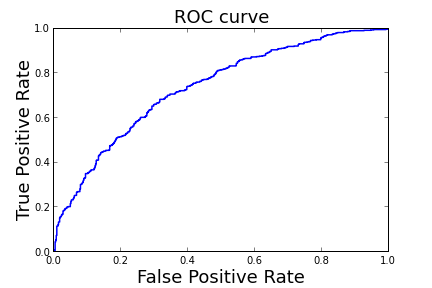
\includegraphics[height=6cm]{doc_en_01.png}

Modelden eksik olan bir sey var; sonraki maci onceki birkac macin ozetinden
tahmin etmeye ugrasiyoruz ama belki bazi takimlar onceki K macta cok zorlu
rakiplerle ugrasmistir, bazilari cok kolay rakiplerle ugrasmistir. Bu
durumda onceki maclarin istatistigi bize tum hikayeyi anlatmayacaktir. 

Bu problemi cozmek icin ayri bir regresyon daha isletebiliriz. Bu regresyon
bir guc siralamasi (power ranking) hesaplayabilir, bu hesap
FIFA/CocaCola'nin enternasyonel takimlar icin yaptigi 
guc siralama hesabina benzer. ABD'de beyzbol ve Amerikan futbolu icin de
benzer bir hesap yapiliyor. 

Guc siralamasi hesabini yaptiktan sonra -tek bir numerik sayi, bazi
takimlar icin daha yuksek bazi takimlar icin daha alcak, ki onun uzerinden
siralama yapilabilsin-, onu bir ozellik olarak lojistik regresyon modeline
dahil edebiliriz. Guc siralamasi esas olarak su tur irdelelerin modelimize
dahilini mumkun kilar; A takimi B'yi yendiyse, B C'yi yendiyse, A buyuk
ihtimalle C takimindan daha iyidir. Bu niye iyi?  Cunku elimizde
yapilabilecek tum maclarin kombinasyonu yok, mac verisi seyrek
(sparse). Ama eldeki birkac mactan bir guc siralamasi hesaplayabilirsek, bu
bize takimlar arasinda, daha once mac oynamamis olsalar bile, otomatik
olarak bir ek bilgi saglayacaktir. 

Siralama hesabi yapildiktan sonra bazi kontrolleri hizla, ciplak gozle
yapabiliriz, mesela sonuca bakariz, eger Wiggan (zayif bir takim) 1.0
degeri almis, Chelsea (guclu bir takim) 0.0 degeri almis ise bir seyler
yanlis demektir.

Tabii buna ragmen bazi takimlara hala uygun siralama veremeyebiliriz,
mesela A,B'yi, B,C'yi yeniyor, sonra veriye gore, C A'yi yeniyor. Bu
sekilde siralayamadigimiz durumda takima 0.5 verip tam ortaya koyacagiz.

Ayrica enternasyonel takimlarin siralamasi cok gurultulu veri oldugu ve
(klup verisinden bile daha) seyrek oldugu icin onu yuzdeliklere (quartiles)
ayirarak gosterecegiz, yani siralamalar 0, .33, .66, or 1.0 olarak
gozukecekler.

Fakat hesap isi bitince, ve bu siralamayi nihai lojistik modele dahil
edince basari oranimizin ziplama yaptigini gorecegiz.

\begin{minted}[fontsize=\footnotesize]{python}
import power
reload(power)
reload(world_cup)
def points_to_sgn(p):
  if p > 0.1: return 1.0
  elif p < -0.1: return -1.0
  else: return 0.0
power_cols = [
  ('points', points_to_sgn, 'points'),
]

power_data = power.add_power(club_data, game_summaries, power_cols)
power_train = power_data.loc[power_data['points'] <> 1] 

# power_train = power_data
(power_model, power_test) = world_cup.train_model(
    power_train, match_stats.get_non_feature_columns())
print "\nRsquared: %0.03g, Power Coef %0.03g" % (
    power_model.prsquared, 
    math.exp(power_model.params['power_points']))

power_results = world_cup.predict_model(power_model, power_test, 
    match_stats.get_non_feature_columns())
power_y = [yval == 3 for yval in power_test['points']]
world_cup.validate(3, power_y, power_results['predicted'], baseline, 
                   compute_auc=True, quiet=False)

print_params(power_model, 8)

plt.plot([0, 1], [0, 1], '--', color=(0.6, 0.6, 0.6), label='Luck')
# Add the old model to the graph
world_cup.validate('old', y, results['predicted'], baseline, 
                   compute_auc=True, quiet=True)
plt.legend(loc="lower right")
plt.savefig('doc_en_02.png')
\end{minted}

\begin{verbatim}
New season 2014
New season 2013
New season 2013
New season 2012
New season 2012
New season 2011

['Blackburn Rovers: 0.000', 'Real Betis: 0.000', 'D.C. United: 0.000',
'Celta de Vigo: 0.004', 'Deportivo de La Coru\xc3\xb1a: 0.009',
'Wolverhampton Wanderers: 0.021', 'Reading: 0.022', 'Real Zaragoza: 0.026',
'Real Valladolid: 0.044', 'Granada CF: 0.062', 'Queens Park Rangers:
0.073', 'Mallorca: 0.089', 'Aston Villa: 0.092', 'Bolton Wanderers: 0.102',
'Osasuna: 0.109', 'Espanyol: 0.112', 'Wigan Athletic: 0.124', 'Sunderland:
0.130', 'Rayo Vallecano: 0.138', 'Almer\xc3\xada: 0.145', 'Levante: 0.148',
'Elche: 0.154', 'Getafe: 0.170', 'Swansea City: 0.192', 'Southampton:
0.197', 'Norwich City: 0.206', 'Toronto FC: 0.211', 'Chivas USA: 0.218',
'West Ham United: 0.220', 'West Bromwich Albion: 0.224', 'Villarreal:
0.231', 'Stoke City: 0.255', 'Fulham: 0.274', 'Valencia: 0.296', 'Valencia
CF: 0.296', 'M\xc3\xa1laga: 0.305', 'Newcastle United: 0.342', 'Sevilla:
0.365', 'Columbus Crew: 0.366', 'Athletic Club: 0.386', 'Liverpool: 0.397',
'Everton: 0.417', 'Philadelphia Union: 0.466', 'Montreal Impact: 0.470',
'Chelsea: 0.530', 'Real Sociedad: 0.535', 'Tottenham Hotspur: 0.551',
'Arsenal: 0.592', 'Houston Dynamo: 0.593', 'FC Dallas: 0.612', 'Chicago
Fire: 0.612', 'Vancouver Whitecaps: 0.615', 'San Jose Earthquakes: 0.632',
'New England Revolution: 0.634', 'Atl\xc3\xa9tico de Madrid: 0.672',
'Colorado Rapids: 0.743', 'Barcelona: 0.759', 'Seattle Sounders FC: 0.781',
'New York Red Bulls: 0.814', 'Sporting Kansas City: 0.854', 'LA Galaxy:
0.882', 'Real Salt Lake: 0.922', 'Manchester City: 0.928', 'Real Madrid:
1.000', 'Manchester United: 1.000', 'Portland Timbers: 1.000'] 

Rsquared: 0.22, Power Coef 2.18
(3) Lift: 1.56 Auc: 0.791
    Base: 0.374 Acc: 0.708 P(1|t): 0.778 P(0|f): 0.667
    Fp/Fn/Tp/Tn p/n/c: 99/248/347/496 595/595/1190
Pozitif ozellikler
power_points      1.177169
is_home           0.787110
opp_op_corners    0.170848
expected_goals    0.058597
opp_cards         0.045538
pass_70           0.036267
avg_goals         0.035456
opp_avg_points    0.033857
dtype: float64

Atilan ozellikler
passes                0
op_pass_80            0
op_expected_goals     0
opp_shots_op_ratio    0
bad_passes            0
pass_ratio            0
opp_pass_op_ratio     0
shots                 0
dtype: float64

Negatif ozellikler
opp_power_points     -0.540688
op_corners           -0.145918
opp_expected_goals   -0.055353
cards                -0.043555
opp_pass_70          -0.034997
opp_avg_goals        -0.034242
avg_points           -0.032748
opp_fouls            -0.022867
dtype: float64
(old) Lift: 1.42 Auc: 0.738
\end{verbatim}

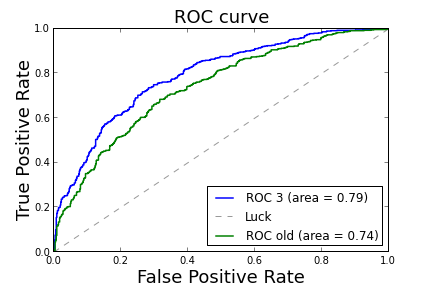
\includegraphics[height=6cm]{doc_en_02.png}

Simdi dunya kupasini tahmin edelim!

Aynen klup verisinde yaptigimiz gibi dunya kupasi icin de benzer
istatistikleri hesaplayabiliriz. Bu durumda elimizde hedefler olmayacak,
yani kimin kazandigini bilemeyecegiz (aslinda bazi dunya kupasi maclarinin
sonucunu biliyoruz, ama tahminlerimizi hicbir maci bilmiyormus gibi
yapalim). Ve tekrar vurgulayalim: klup verisiyle egittigimiz modeli
kullanarak dunya kupasini tahmin edecegiz. Yani model ve tahmin tamamen
farkli takimlar uzerinden yapilacak!

\verb!features.get_wc_features()! bize tum dunya kupasi maclari icin
gereken ozellikleri yaratip dondurecektir.

\begin{minted}[fontsize=\footnotesize]{python}
import world_cup
import features
reload(match_stats)
reload(features)
reload(world_cup)
wc_data = world_cup.prepare_data(features.get_wc_features(history_size))
wc_labeled = world_cup.prepare_data(features.get_features(history_size))
wc_labeled = wc_labeled[wc_labeled['competitionid'] == 4]
wc_power_train = game_summaries[game_summaries['competitionid'] == 4].copy()
\end{minted}

Ev sahasi avantaji

Klup verisi ile dunya kupasi verisi arasindaki bazi farklardan biri budur:
dunya kupasinda, mac basina ev sahibi olmak, deplasmanda olmak ne demektir?
Resmi olarak tek ev sahibi tum 2014 kupasina ev sahipligi yapan
Brezilya'dir, o zaman sadece Brezilya mi mac basina sadece ev sahibi
olabilir? Bu pek akla yatkin gelmiyor. 

Belki diger Latin Amerika takimlarini da ev sahibi olarak gorebiliriz..?
Diger bazi modeller \verb!is_home!'u sadece Brezilya'ya vermis, sonra ayni
kitadaki diger takimlara da 'azicik' ev sahipligi vermisler, cunku
istatistiklere gore bu takimlar kendi kitalarinda daha iyi performans
gosteriyorlarmis, vs.

Biz daha degisik bir model kullanacagiz, bu model belki biraz
subjektif.. Biz \verb!is_home! ogesine 0.0 ila 1.0 arasinda bir deger
atayacagiz, ve bu degerin buyuklugu o takimin taraftarlarinin hem sayi, hem
de destek enerjisi uzerinden olculecek. Bunu yapmamizin sebebi ilk turlarda
goruldugu uzere, taraftarinin daha iyi destekledigi takimlarin digerlerine
gore daha iyi performans gostermesi. Mesela Sili'nin taraftari takimini
muthis destekledi, Ispanya taraftari orali bile olmadi, Sili-Ispanya macini
Sili 2-0 kazandi. Bunun gibi pek cok mac gozlemledik, cogunda guney Amerika
takimlari vardi, ama cok taraftar gonderen takimlar da vardi, mesela
Meksika. Ya da ABD vardi, cok taraftari vardi ama sessizdiler, onlar daha
dusuk skorlar aldilar.

\begin{minted}[fontsize=\footnotesize]{python}
import pandas as pd
wc_home = pd.read_csv('wc_home.csv')

def add_home_override(df, home_map):
  for ii in xrange(len(df)):
    team = df.iloc[ii]['teamid']
    if team in home_map:
        df['is_home'].iloc[ii] = home_map[team]
    else:
        # If we don't know, assume not at home.
        df['is_home'].iloc[ii] = 0.0
        
home_override = {}
for ii in xrange(len(wc_home)):
    row = wc_home.iloc[ii]
    home_override[row['teamid']] = row['is_home']

# Add home team overrides.
add_home_override(wc_data, home_override)    
\end{minted}

Dunya Kupasi Guc Siralamasi

Bu hesabin dunya kupasi verisi uzerinde yapilmasi lazim, cunku guc
siralamasi o takimlarin arasindaki maclara dayanilarak yapilan bir
hesap. Bu maclar ise, dunya kupasi takimlari baglaminda, oldukca seyrek
cunku bazi takimlar bazi takimlarla neredeyse onyildir oynamamis. Cogu
Avrupa takimi mesela guney Amerika takimiyla oynamamis, Asyali takimlarla
daha bile az oynamis. Klup bazinda kullandigimiz ayni numarayi burada da
kullanabiliriz, ama basarisizliga hazir olmak lazim! 

Hesap altta

\begin{minted}[fontsize=\footnotesize]{python}
# When training power data, since the games span multiple competitions, 
# just set is_home to 0.5
#
# Otherwise when we looked at games from the 2010 world cup, we'd think 
# Brazil was still at home instead of South Africa.

wc_power_train['is_home'] = 0.5
wc_power_data = power.add_power(wc_data, wc_power_train, power_cols)

wc_results = world_cup.predict_model(power_model, wc_power_data, 
    match_stats.get_non_feature_columns())
\end{minted}

\begin{verbatim}
New season 2013
New season 2009
New season 6
['Australia: 0.000', 'Serbia: 0.016', 'USA: 0.017', 'Cameroon: 0.035',
'Iran: 0.081', 'Croatia: 0.180', 'Nigeria: 0.204', "C\xc3\xb4te d'Ivoire:
0.244", 'Costa Rica: 0.254', 'Algeria: 0.267', 'Paraguay: 0.277',
'Honduras: 0.279', 'Slovakia: 0.281', 'Greece: 0.284', 'Switzerland:
0.291', 'Ecuador: 0.342', 'Uruguay: 0.367', 'Sweden: 0.386', 'Japan:
0.406', 'Mexico: 0.409', 'Chile: 0.413', 'Colombia: 0.438', 'England:
0.460', 'Belgium: 0.467', 'Ukraine: 0.470', 'Portugal: 0.487', 'Ghana:
0.519', 'South Korea: 0.532', 'France: 0.648', 'Spain: 0.736', 'Argentina:
0.793', 'Italy: 0.798', 'Brazil: 0.898', 'Netherlands: 0.918', 'Germany:
1.000'] 
\end{verbatim}

Guc sirasi da ayri bir lojistik regresyon aslinda, \verb!power.py! icinde
biz bu regresyona giren matris ve etiketleri hesap yapilmadan once cekip
cikarttik, ve bir dosyaya kaydettirdik. Bakarsak,

\begin{minted}[fontsize=\footnotesize]{python}
games = pd.read_csv('/tmp/games.csv')
outcomes = pd.read_csv('/tmp/outcomes.csv')
\end{minted}

Herhangi bir satira goz atalim,

\begin{minted}[fontsize=\footnotesize]{python}
print 'mac', games[100:101]
print 'sonuc', outcomes[100:101]
\end{minted}

\begin{verbatim}
mac      1041  1042  114  1161  118  119  1215  1216  1219  1221  1223  1224  \
100     0     0    0     0    0    0     0     0     0     0     0     0   

     1264  1266  1794  1801  1804  357  359  360  361  364  365  366  367  \
100     0     0     0     0     0    0    0    0    0    0    0    0    0   

     368     369     494  497  507  510  511  517  522  535  536  537  575  \
100    0 -1.5625  1.5625    0    0    0    0    0    0    0    0    0    0   

     596  614  632  659  830  831  832  835  837  838  847  
100    0    0    0    0    0    0    0    0    0    0    0  
sonuc      0.0
100    0
\end{verbatim}

Yani guc siralamasi lojistik regresyonuna girdi olan matrisin her satiri
ayri bir mac, her kolonu ise ayri bir takim. Mac yapan iki takimin
degerleri olacak, digerleri sifir olacak. Ustteki satir mesela, 369. takim
ve rakipte 494. takim icin,

\begin{minted}[fontsize=\footnotesize]{python}
raw_games = pd.read_csv('results-20140714-124014.csv')
tmp = raw_games[(raw_games['teamid'] == 369) & (raw_games['op_teamid'] == 494)]
tmp = tmp[['teamid','team_name','op_team_name','is_home','points']]
print tmp
\end{minted}

\begin{verbatim}
      teamid team_name op_team_name  is_home  points
4231     369   Denmark     Cameroon        0       3
\end{verbatim}

Danimarka Kamerun macina aitmis. Bu macta Danimarka kazandi, ev sahibi
Kamerun. Simdi burada birkac onemli takla atiliyor, Google veri bilimcileri
lojistik regresyonda, girdi olarak, deplasman takimina her mac basinda
otomatik olarak eksi bir deger veriyorlar, ev sahibine arti deger
veriyorlar. Etiket ise 'ev sahibi kazandi mi?' sorusunun cevabi.

Ev sahibi olup kazanmak daha kolay, regresyon baglaminda arti degere sahip
olursaniz, az bir katsayi modeli uydurmaya yeterli olabilir, pozitife hemen
yaklasiriz. Diger yandan deplasman takimi ne kadar iyi oynarsa, onun buyuyen
katsayisi eksi degerini o kadar arttirir, ve ev sahibinin artisini (onun
ogesi carpi katsayisi yani) eksilterek kaybetme durumuna yaklastirir.

Kotu oynayan deplasman takiminin eksi degeri eksi katsayi ile carpilir, ve
daha buyuk bir arti sayiya sebebiyet verir, ev sahibinin kazanmasi durumunu
guclendirir. 

Katsayilari dogal olarak bir takimin ne kadar iyi oldugunu gosterecektir. 

Tabii regresyona pek cok satir verilecek, Kamerun birden fazla satirda
ortaya cikabilecek, bazen arti degerli olarak (ev sahibi) bazen eksi
degerli olarak (deplasman). 

Itiraf etmek gerekir ki veri bilimi baglaminda ustteki teknik, model,
dusunce tarzi dahiyane bir yaklasim. Bu is kolunun ruhunu gostermesi
bakimindan son derece onemli bir ornek. Hem ustteki veri temsili, hem de
regresyonun kodlanmasinda ceyrekliklere ayirmak, az veri oldugu icin
yaklasiksallik (convergence) olmayabilir diye degisik parametrelerle
regresyonu birkac kez isletmek, bunu yaklasiksallik olana kadar yapmak,
muthis. Iste alanimizin puf noktalari burada gosteriliyor.

Tahmin

Nihayet hazirlandigimiz ana geldik. Simdi dunya kupasi maclarini tahmin
edelim. Birkac kolon gosterecegiz:

\verb!predicted!: Yuzde kac ihtimalle (ismi ilk gelen) takimin kazanacagi

\verb!points!: Gercekten ne oldugu. Oynanmayan mac \verb!NaN!. Dikkat,
penalti atislarina giden maclar esitlik olarak gosterilecek.

Ama bir dakika! Bu sonuclar daha once gosterdiginiz [Google tahminleri
kastediliyor] tahminlerinden degisik! Bunun sebepleri sunlar: Bazi hatalari
tamir ettik, yani kod degisti. Ilk model mesela uzayan maclar yuzunden
kabaran istatistiklerin durumunu hesaba almiyordu.

Ikinci sebep, model sonu belli (deterministik) degil, egitim verisi icin
verinin belli bir kismini rasgele olarak seciyoruz, bu sebeple sonuclar bir
hesaptan digerine degisik cikabiliyor (ki bazen sonuclar cok degisik
olabiliyor). Not: Aslinda bu kod degistirilerek rasgelelik icinden tamamen
cikartilabilir (ev odeviniz!). 

16. turu tahmin ederken mesela onceki 3 maci, ceyrek finaller icin onceki
4, yarifinaller icin 5, ve finaller icin onceki 6 maci kullandik [biz bu
dokumanda onceki 3 maci kullandik, \verb!history_size! parametresiyle
oynayarak degisik sonuclar kontrol edilebilir].

\begin{minted}[fontsize=\footnotesize]{python}
pd.set_option('display.max_rows', 5000)
pd.set_option('display.max_columns', 500)
pd.set_option('display.width', 1000)

wc_with_points = wc_power_data.copy()
wc_with_points.index = pd.Index(
    zip(wc_with_points['matchid'], wc_with_points['teamid']))
wc_labeled.index = pd.Index(
    zip(wc_labeled['matchid'], wc_labeled['teamid']))
wc_with_points['points'] = wc_labeled['points']

wc_pred = world_cup.extract_predictions(wc_with_points, 
                                        wc_results['predicted'])

# Reverse our predictions to show the most recent first.
wc_pred.reindex(index=wc_pred.index[::-1])
# Show our predictions for the games that have already happenned.
print wc_pred
\end{minted}

\begin{verbatim}
        team_name   op_team_name  predicted       expected         winner  points
0       Argentina        Germany  46.070814        Germany             NA     NaN
1     Netherlands         Brazil  42.833863         Brazil             NA     NaN
2     Netherlands      Argentina  48.641542      Argentina           draw       1
3         Germany         Brazil  44.011593         Brazil        Germany       3
4      Costa Rica    Netherlands  14.442625    Netherlands           draw       1
5         Belgium      Argentina  18.596031      Argentina      Argentina       0
6        Colombia         Brazil  23.890421         Brazil         Brazil       0
7         Germany         France  75.116349        Germany        Germany       3
8             USA        Belgium  32.400646        Belgium        Belgium       0
9     Switzerland      Argentina  19.272768      Argentina      Argentina       0
10        Algeria        Germany   5.926496        Germany        Germany       0
11        Nigeria         France   8.694729         France         France       0
12         Greece     Costa Rica  40.448104     Costa Rica           draw       1
13         Mexico    Netherlands  20.402491    Netherlands    Netherlands       0
14        Uruguay       Colombia  46.480264       Colombia       Colombia       0
15          Chile         Brazil  26.574916         Brazil           draw       1
16        Germany            USA  91.980986        Germany        Germany       3
17          Ghana       Portugal  49.051707       Portugal       Portugal       0
18    Switzerland       Honduras  60.223070    Switzerland    Switzerland       3
19         France        Ecuador  84.538857         France           draw       1
20      Argentina        Nigeria  88.491450      Argentina      Argentina       3
21  Côte d'Ivoire         Greece  61.074502  Côte d'Ivoire         Greece       0
22        Uruguay          Italy  32.685428          Italy        Uruguay       3
23        England     Costa Rica  63.457326        England           draw       1
24         Brazil       Cameroon  94.788074         Brazil         Brazil       3
25         Mexico        Croatia  78.020214         Mexico         Mexico       3
26          Spain      Australia  90.521542          Spain          Spain       3
27          Chile    Netherlands  28.342133    Netherlands    Netherlands       0
28       Portugal            USA  65.457259       Portugal           draw       1
29        Algeria    South Korea  17.376285    South Korea        Algeria       3
30          Ghana        Germany  14.588539        Germany           draw       1
31           Iran      Argentina   5.193843      Argentina      Argentina       0
32        Ecuador       Honduras  53.848926        Ecuador        Ecuador       3
33         France    Switzerland  78.659381         France         France       3
34     Costa Rica          Italy  24.836756          Italy     Costa Rica       3
35         Greece          Japan  44.355013          Japan           draw       1
36        England        Uruguay  61.012694        England        Uruguay       0
37        Croatia       Cameroon  40.212875       Cameroon        Croatia       3
38          Chile          Spain  42.624474          Spain          Chile       3
39    Netherlands      Australia  93.535889    Netherlands    Netherlands       3
40         Mexico         Brazil  20.372064         Brazil           draw       1
41            USA          Ghana  39.500993          Ghana            USA       3
42        Nigeria           Iran  53.813244        Nigeria           draw       1
43       Portugal        Germany  15.337884        Germany        Germany       0
44       Honduras         France  22.953848         France         France       0
45        Ecuador    Switzerland  59.987076        Ecuador    Switzerland       0
46          Japan  Côte d'Ivoire  51.528885          Japan  Côte d'Ivoire       0
47          Italy        England  68.767968          Italy          Italy       3
48     Costa Rica        Uruguay  45.347946        Uruguay     Costa Rica       3
49      Australia          Chile  19.487987          Chile          Chile       0
50    Netherlands          Spain  60.493928    Netherlands    Netherlands       3
51       Cameroon         Mexico  30.018950         Mexico         Mexico       0
52        Croatia         Brazil   6.268704         Brazil         Brazil       0
53          Spain    Netherlands  35.602227    Netherlands          Spain       3
54        Germany        Uruguay  76.467450        Germany        Germany       3
55          Spain        Germany  29.438134        Germany          Spain       3
56    Netherlands        Uruguay  71.342186    Netherlands    Netherlands       3
57          Spain       Paraguay  83.007655          Spain          Spain       3
58        Germany      Argentina  42.635127      Argentina        Germany       3
59          Ghana        Uruguay  41.784682        Uruguay           draw       1
60         Brazil    Netherlands  60.821972         Brazil    Netherlands       0
61       Portugal          Spain  23.464891          Spain          Spain       0
62          Japan       Paraguay  61.278000          Japan           draw       1
63          Chile         Brazil  24.459600         Brazil         Brazil       0
64       Slovakia    Netherlands  12.082967    Netherlands    Netherlands       0
65         Mexico      Argentina  17.626748      Argentina      Argentina       0
66        England        Germany  20.763176        Germany        Germany       0
67          Ghana            USA  71.310871          Ghana          Ghana       3
68    South Korea        Uruguay  45.148588        Uruguay        Uruguay       0
69         Brazil       Portugal  81.610878         Brazil           draw       1
70        Germany          Ghana  81.621494        Germany        Germany       3
71         Serbia      Australia  38.204905      Australia      Australia       0
72  Côte d'Ivoire         Brazil  10.186423         Brazil         Brazil       0
73      Australia          Ghana  23.702414          Ghana           draw       1
74          Japan    Netherlands  10.773998    Netherlands    Netherlands       0
75         Serbia        Germany   4.731113        Germany         Serbia       3
76         Mexico         France  42.801515         France         Mexico       3
77    South Korea      Argentina  15.255040      Argentina      Argentina       0
78    Switzerland          Spain  18.747704          Spain    Switzerland       3
79       Portugal  Côte d'Ivoire  65.031075       Portugal           draw       1
80       Paraguay          Italy  12.288896          Italy           draw       1
81      Australia        Germany   7.395354        Germany        Germany       0
82          Ghana         Serbia  83.682899          Ghana          Ghana       3
83            USA        England  34.763699        England           draw       1
84         France          Italy  28.651132          Italy           draw       1
85       Portugal        Germany  14.833907        Germany        Germany       0
86         France       Portugal  72.141913         France         France       3
87          Italy        Germany  33.364112        Germany          Italy       3
88         France         Brazil  22.742882         Brazil         France       3
89       Portugal        England  49.550454        England           draw       1
90        Ukraine          Italy  28.378865          Italy          Italy       0
91      Argentina        Germany  46.801014        Germany           draw       1
92         France          Spain  47.126654          Spain         France       3
93          Ghana         Brazil   9.144470         Brazil         Brazil       0
94        Ukraine    Switzerland  62.637340        Ukraine           draw       1
95      Australia          Italy   8.365416          Italy          Italy       0
96    Netherlands       Portugal  70.231295    Netherlands       Portugal       0
97        Ecuador        England  34.379086        England        England       0
98         Mexico      Argentina  29.233199      Argentina      Argentina       0
99         Sweden        Germany  10.914079        Germany        Germany       0
\end{verbatim}


Kodlar

\inputminted[fontsize=\footnotesize]{python}{world_cup.py}

\inputminted[fontsize=\footnotesize]{python}{power.py}

\inputminted[fontsize=\footnotesize]{python}{features.py}

\inputminted[fontsize=\footnotesize]{python}{match_stats.py}

Kaynaklar

[1] \url{http://googlecloudplatform.blogspot.de/2014/07/google-cloud-platform-goes-8-for-8-in-soccer-predictions.html}

[2] \url{https://github.com/GoogleCloudPlatform/ipython-soccer-predictions}

[3] \url{http://nbviewer.ipython.org/github/GoogleCloudPlatform/ipython-soccer-predictions/blob/master/predict/wc-final.ipynb}

[4] \url{http://sayilarvekuramlar.blogspot.com/2014/07/dunya-kupasini-tahmin-lojistik-regresyon.html}

\end{document}
